\begin{solution}
\begin{enumerate}
\item {[10 points]} We have that
\begin{eqnarray*}
   \norm{f-f_N}^2 &=& \left( f-f_N, f-f_N\right) \\[0.5em]
 &=& \left( f - \sum_{n=1}^N \alpha_n \psi_n,
                           f - \sum_{m=1}^N \alpha_m \psi_m\right) \\[0.5em]
 &=& \left( f - \sum_{n=1}^N \alpha_n \psi_n, f\right) 
              -\sum_{m=1}^N \alpha_m \left( f - \sum_{n=1}^N \alpha_n \psi_n,   \psi_m\right) \\[0.5em]
 &=& \left(f,f\right) - \sum_{n=1}^N \alpha_n\left( \psi_n, f\right) 
              - \sum_{m=1}^N \alpha_m\left( f,   \psi_m\right) 
           +  \sum_{m=1}^N \alpha_m \sum_{n=1}^N \alpha_n (\psi_n, \psi_m) \\[0.5em]
 &=& (f,f) - \sum_{n=1}^N \alpha_n (\psi_n, f) 
           - \sum_{m=1}^N \alpha_m (f,\psi_m)
           + \sum_{n=1}^N \alpha_n^2  (\psi_n, \psi_n)\\[0.5em]
 &=& (f,f) - \sum_{n=1}^N \alpha_n (\psi_n, f) 
           - \sum_{m=1}^N \alpha_m (f,\psi_m)
           + \sum_{n=1}^N \alpha_n^2\\[0.5em]
 &=& (f,f) - \sum_{n=1}^N \alpha_n^2  
           - \sum_{m=1}^N \alpha_m^2 
           + \sum_{n=1}^N \alpha_n^2 \\[0.5em]
 &=& (f,f) - \sum_{n=1}^N \alpha_n^2 \\[0.5em]
 &=& \norm{f}^2 - \sum_{n=1}^N \alpha_n^2,
\end{eqnarray*}
where at each equal sign we have used:
(1) the definition of the norm $\norm{\cdot}$;
(2) the definition of $g_N$;
(3) linearity of the inner product in the second argument;
(4) linearity of the inner product in the first argument;
(5) the fact that $(\psi_n,\psi_m) = 0$ if $n\ne m$, for $m,n=1,2,\ldots,N$, since $\left\{\psi_1,\ldots,\psi_N\right\}$ is orthonormal with respect to the inner product $(\cdot,\cdot)$;
(6) the fact that $(\psi_n,\psi_n) = 1$, for $n=1,2,\ldots,N$, since $\left\{\psi_1,\ldots,\psi_N\right\}$ is orthonormal with respect to the inner product $(\cdot,\cdot)$;
(7) the fact that $(f,\psi_n) = (\psi_n,f) = \alpha_n$;
(8) algebra;
(9) the definition of the norm $\norm{\cdot}$.
\\
\item {[10 points]} First calculate the norm of $f$
 \[
\norm{f}^2=\int_0^1\left(f(x)\right)^2\,dx=\int_0^1 x^2 (1-x)^2 \,dx=\frac{1}{30}.
\]
Then
\[
\norm{f-f_N}^2 = \norm{f}^2 - \sum_{n=1}^N \alpha_n^2,
\]
where
\[
\alpha_n={2 \sqrt{2} \over n^3 \pi^3} \left(1-\left(-1\right)^n\right).
\]
and so
\[
\norm{f-f_N}^2 = \frac{1}{30} - \sum_{n=1}^N \alpha_n^2.
\]
The requested plots are shown below. 
\begin{figure}
\centering
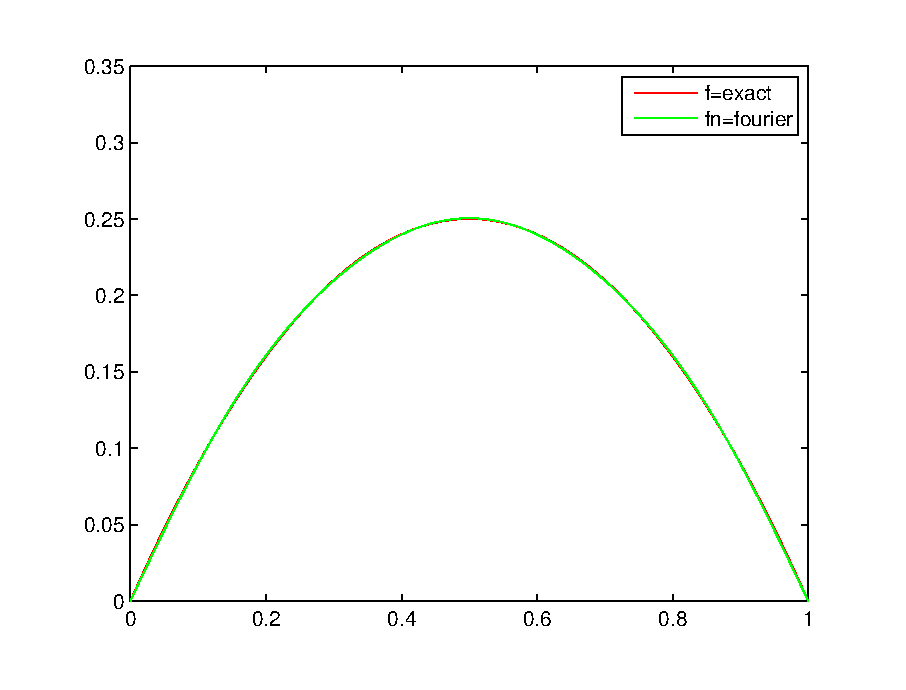
\includegraphics[scale=0.9]{ffn}
\vspace{-.5cm}
\caption{Comparison of the true function $f(x)$ and $f_N(x)$ for $N = 5$}
\end{figure}

\begin{figure}
\centering
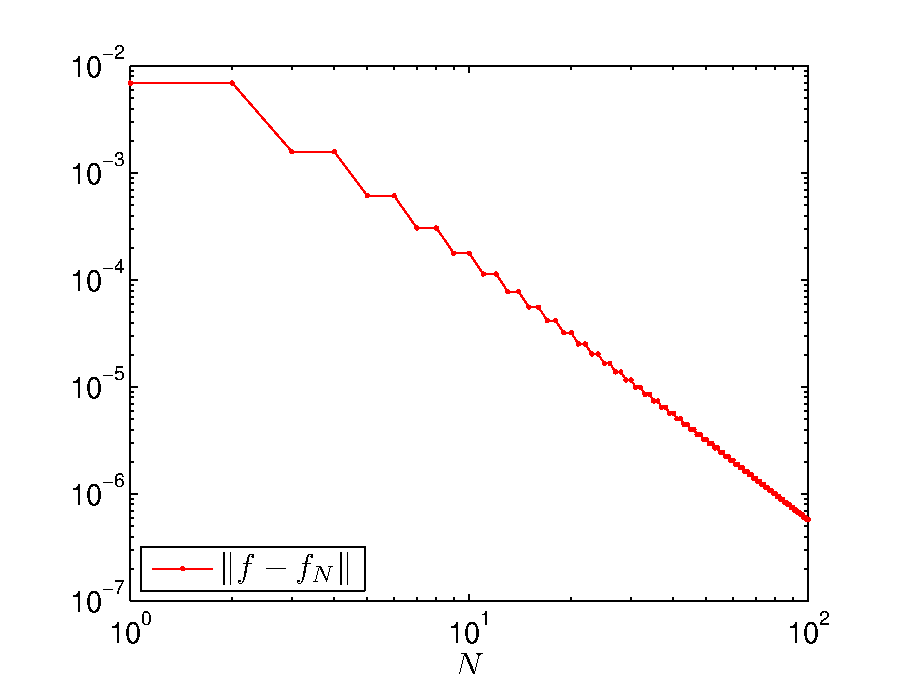
\includegraphics[scale=0.9]{ffnnorm}
\vspace{-.4cm}
\caption{Norm of the error for $N=1,2 \cdots,100$ on a log-log scale}
\end{figure}


\newpage
The codes that produced the plots are shown below, respectively.
\lstinputlisting{HW6_3b.m}
\lstinputlisting{HW6_3b2.m}

\item {[12 points]} The best approximation to the function $$f(x) = 1 - x$$ using orthonormal eigenfunction $\phi_n (x)$ can be written as follows
\[
f_N (x) = \sum_{n=1}^N \alpha _n \phi_n (x)\]
where
\[
\alpha_n= \ip{f, \phi_n}=\int_0^1 (1-x) \sqrt{2}\sin(n \pi x) \, dx= \sqrt{2} \left[\frac{n \pi (x-1) \cos (n \pi x) - \sin(n \pi x)}{n^2 \pi^2}\right]_0^1 = \frac{\sqrt{2}}{n \pi}
\]
Now, calculate the norm of $f$
 \[
\norm{f}^2=\int_0^1\left(f(x)\right)^2\,dx=\int_0^1(1-x)^2 \,dx=\frac{1}{3}.
\]
Then
\[
\norm{f-f_N}^2 = \norm{f}^2 - \sum_{n=1}^N \alpha_n^2,
\]
and so
\[
\norm{f-f_N}^2 = \frac{1}{3} - \sum_{n=1}^N \alpha_n^2.
\]
The requested plots are shown below. 


\begin{figure}
\centering
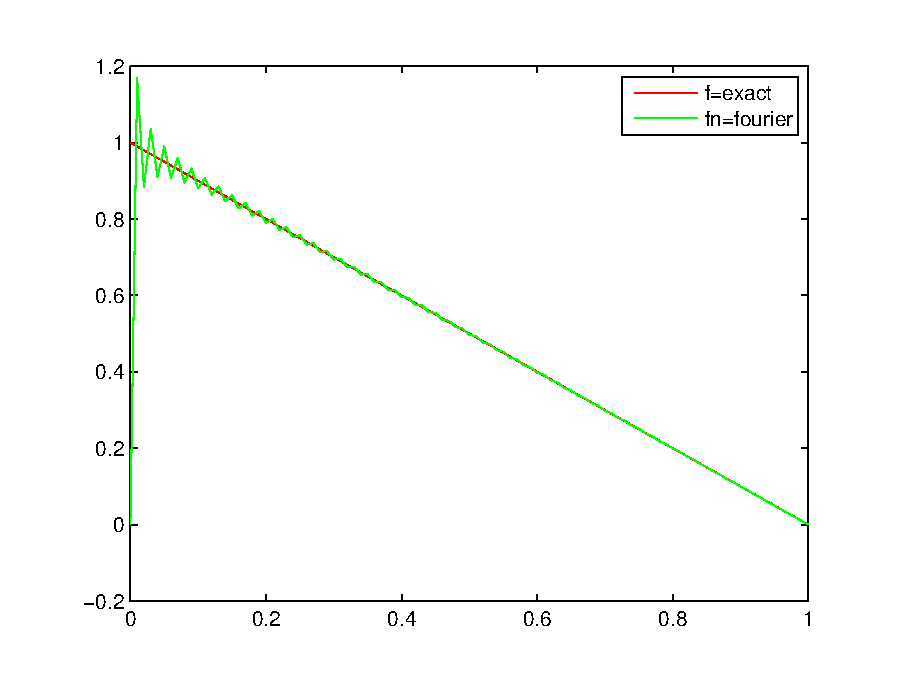
\includegraphics[scale=0.9]{ffnc}
\vspace{-.5cm}
\caption{Comparison of the true function $f(x)$ and $f_N(x)$ for $N = 100$}
\end{figure}

\begin{figure}
\centering
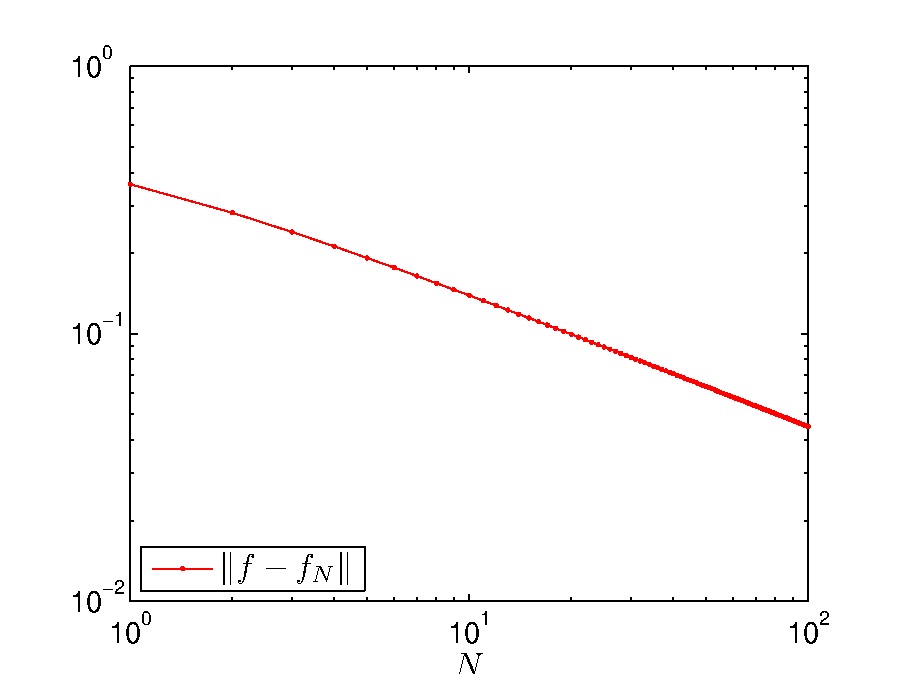
\includegraphics[scale=0.9]{ffnnormc}
\vspace{-.4cm}
\caption{Norm of the error for $N=1,2 \cdots,100$ on a log-log scale}
\end{figure}

\newpage
The codes that produced the plots are shown below, respectively.

\lstinputlisting{HW6_3c.m}
\lstinputlisting{HW6_3c2.m}

\end{enumerate}

\end{solution}
